\chapter{Numerical Results}

The above calculations were one for the case of one dimension, however, such one-dimensional features can be achieved by applying two transversal lattices of large depth in the two remaining dimensions. This effectively decouples neighboring sites in the transverse directions, thus creating a lattice consisting of an array of tubes. However, this does affect the $U$-parameter (equation \ref{eq:BH_U}), as one has to integrate over the transverse directions as well.
The following calculations reflects the setup described in \cite{FrankBloch}.  Thus, the species of atoms used is Rubidium 87, the optical lattice is created using a wavelength of $\lambda = 1064 \mathrm{nm}$, and the transverse lattice depth is $20 E_r$.

\begin{figure}[t]
    \centering
    \begin{subfigure}[t]{0.49\textwidth}
        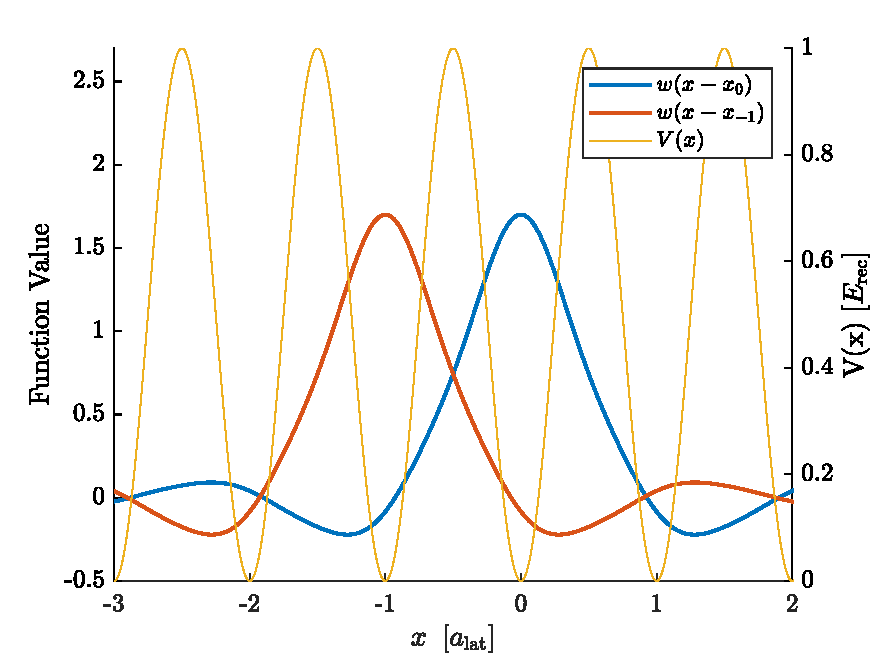
\includegraphics[width=\textwidth]{Figures/WannierPlot1.pdf}
    \end{subfigure}
    ~
    \begin{subfigure}[t]{0.49\textwidth}
        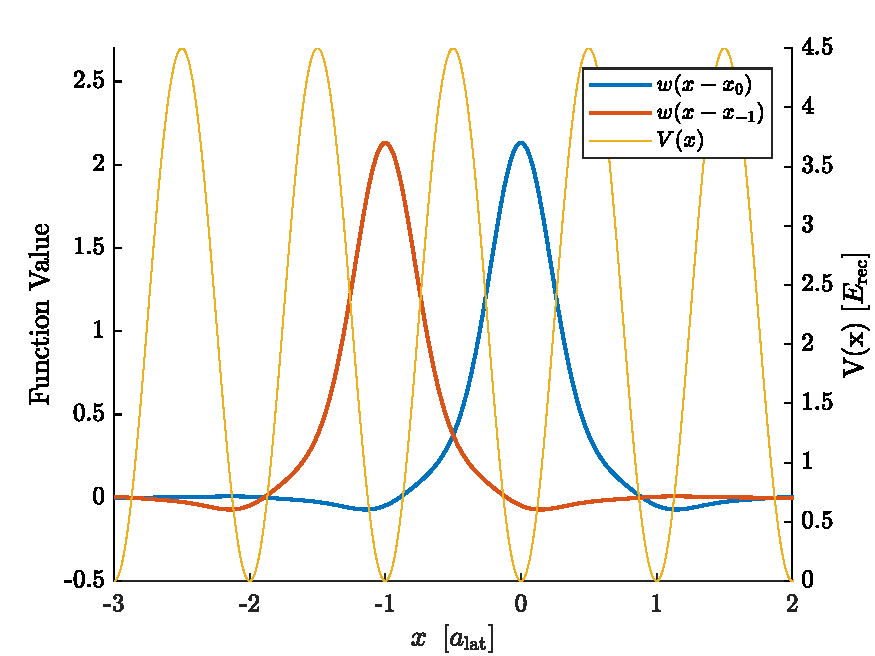
\includegraphics[width=\textwidth]{Figures/WannierPlot2.pdf}
    \end{subfigure}
    ~
    \begin{subfigure}[t]{0.49\textwidth}
        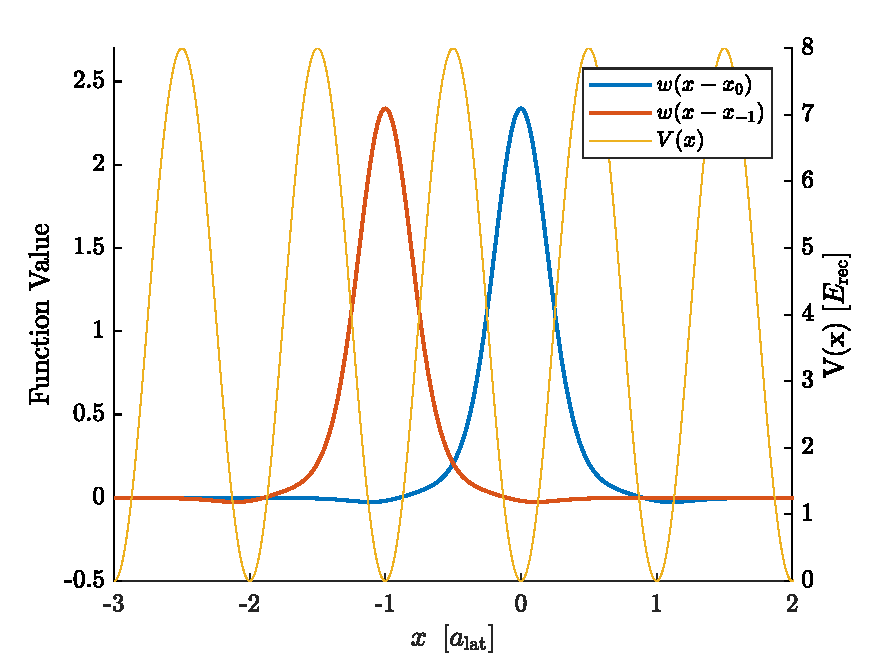
\includegraphics[width=\textwidth]{Figures/WannierPlot3.pdf}
    \end{subfigure}
    ~
    \begin{subfigure}[t]{0.49\textwidth}
        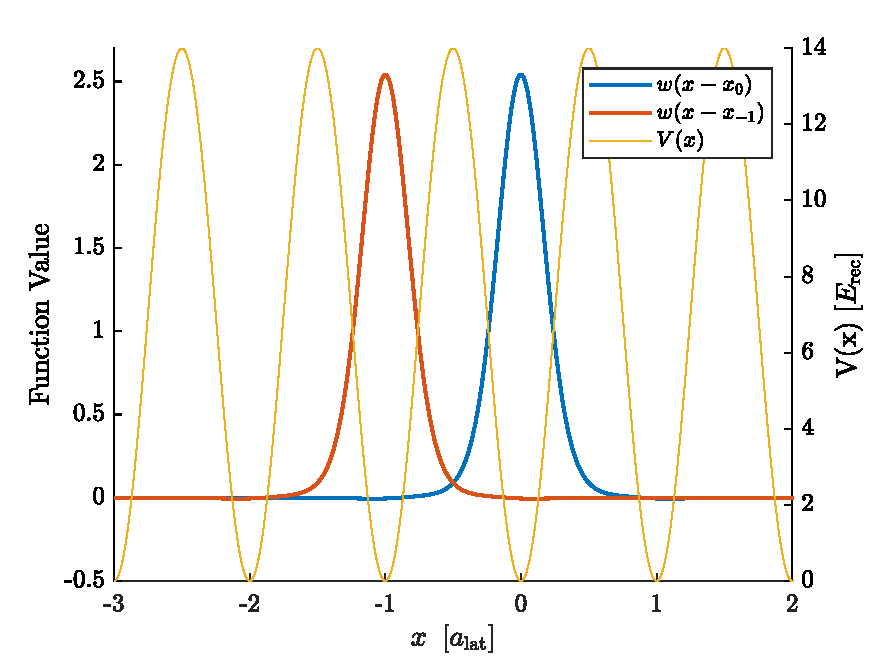
\includegraphics[width=\textwidth]{Figures/WannierPlot4.pdf}
	\end{subfigure}
	\caption{\textit{Calculated Wannier functions for lattice depths $V_0 = 1 E_{\mathrm{r}} , \; 4.5 E_{\mathrm{r}} , \; 8 E_{\mathrm{r}} ,$ and $14 E_{\mathrm{r}}$.}}
	\label{fig:numWannier}    
\end{figure}
Figure \ref{fig:numWannier} displays Wannier functions for two neighboring sites calculated using equation \ref{eq:wannierrescaled} for various lattice depths. For $V_0 = 1 E_{\mathrm{r}}$ the Wannier functions do not show a high degree of localization, as they extend over multiple sites. Thus, there is a large overlap between neighboring functions resulting in a large value of the $J$-parameter (equation \ref{eq:BH_J}). As the lattice becomes deeper, the Wannier functions become more localized: Within the tight binding limit the Wannier functions only overlap with their nearest neighbors. Hence, the kinetic term in the Bose-Hubbard model takes only nearest-neighbor hopping into account. At large lattice depths the Wannier functions barely overlap and are well approximated by Gaussians. As almost no interaction between sites takes place, the lattice turns into an array of decoupled harmonic oscillators. Hence, the Wannier functions tends towards Gaussians, as these are the eigenstates of the harmonic oscillator. 
\begin{figure}[h]
	\centering
	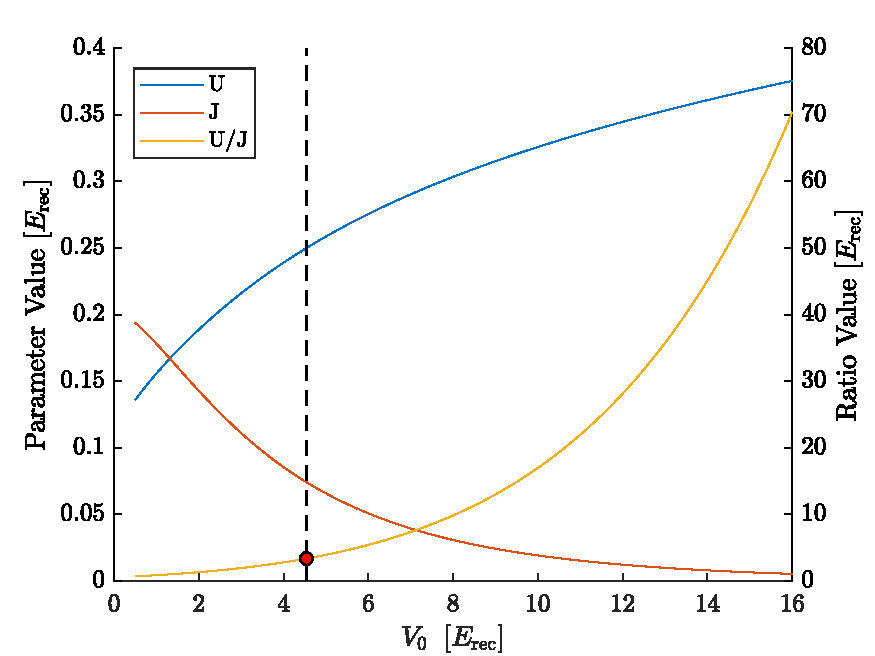
\includegraphics[width=0.9\textwidth]{Figures/parameters.pdf}
	\caption{\textit{Bose-Hubbard parameters calculated as function of lattice depth using a transversal confinement of $V_{0,t} = 20 E_r$. The vertical dashed line marks the critical point of the SF-MI phase transition in 1D. }}
	\label{fig:params}
\end{figure}
Figure \ref{fig:params} displays the evolution of the Bose-Hubbard parameters as the lattice depth is increased along the final dimension. While $J$ decreases as expected, the stronger confinement and following increase in localization of the Wannier functions results in an increase in $U$. In total, the fraction $U/J$ increases rapidly with the lattice depth. The critical point of the quantum phase transition from Superfluid to Mott-Insulator for one dimension is $\left( U/J \right)_{\mathrm{crit}} = 3.37$ \cite{Kuhner2000}, which is marked in figure \ref{fig:params} by the point and the dashed line. 